%!TEX root = ../thesis.tex

\chapter{Test and Validation}

\ifpdf
    \graphicspath{{Chapters/Figs/Raster/}{Chapters/Figs/PDF/}{Chapters/Figs/}}
\else
    \graphicspath{{Chapters/Figs/Vector/}{Chapters/Figs/}}
\fi

%********************************** % Intro *****************************************
%Il framework che è stato sviluppato (\ref{sec:DevelopedFramework}) prevede 3 fasi, lo sviluppo del modello, lo scheduling e la generazione di codice. Per dimostrare il funzionamento del framework viene presentato un esempio.

%********************************** % Section  **************************************
\section{Example model}
The example from the EMC2 project not relatively straightforward for showing the tool capabilities. Therefore, as test example model, let consider a quad-rotor flight control with a pan/tilt camera on it shown in figure \ref{fig:exampleModel}. The pan and tilt camera is moved by two servo motors controlled by two PID that do not communicate with the flight control of the drone. The adopted drone control scheme is taken from \cite{PeterCorke2011} with minor changes introduced to comply with our design restrictions. The original model in \cite{PeterCorke2011} contains different functional loops, each of them has been included in a Simulink subsystem representing a task. The quad-rotor and the motors dynamics that has been used during the simulation have been substituted to enable code generation. The \emph{Quadrotor} block contains the control for its motors and the interface to its sensors. The motors blocks are interface blocks to their encoders. The pan/tilt motor control has a sample time of $0.05$ seconds, the drone flight control a sample time of $0.1$ seconds and the quad-rotor block a sample time of $0.01$ seconds.
\begin{figure}[htbp] 
\centering    
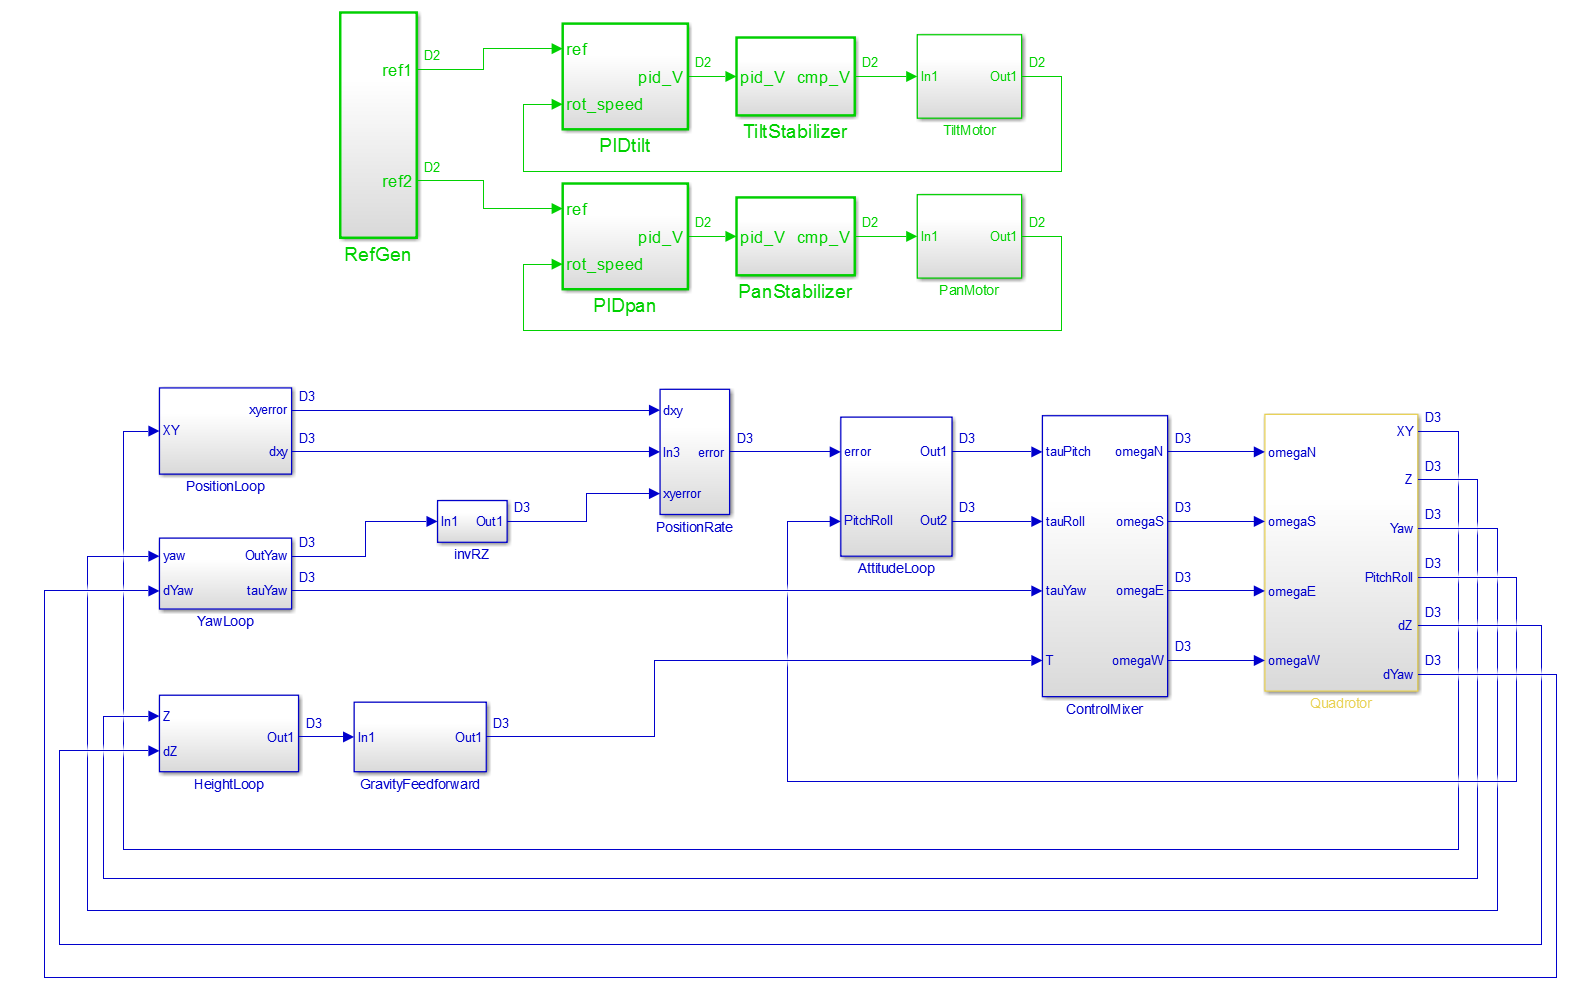
\includegraphics[width=0.9\textwidth]{CompiledModel}
\caption{Example Model}
\label{fig:exampleModel}
\end{figure}

This example is oriented to demonstrate the capabilities of the framework, so it does not focus on the performance of the controller. When the model is ready to be used, the framework GUI (fig. \ref{fig:GUI}) can be started with the command \verb|START|. 
\begin{figure}[htbp] 
\centering    
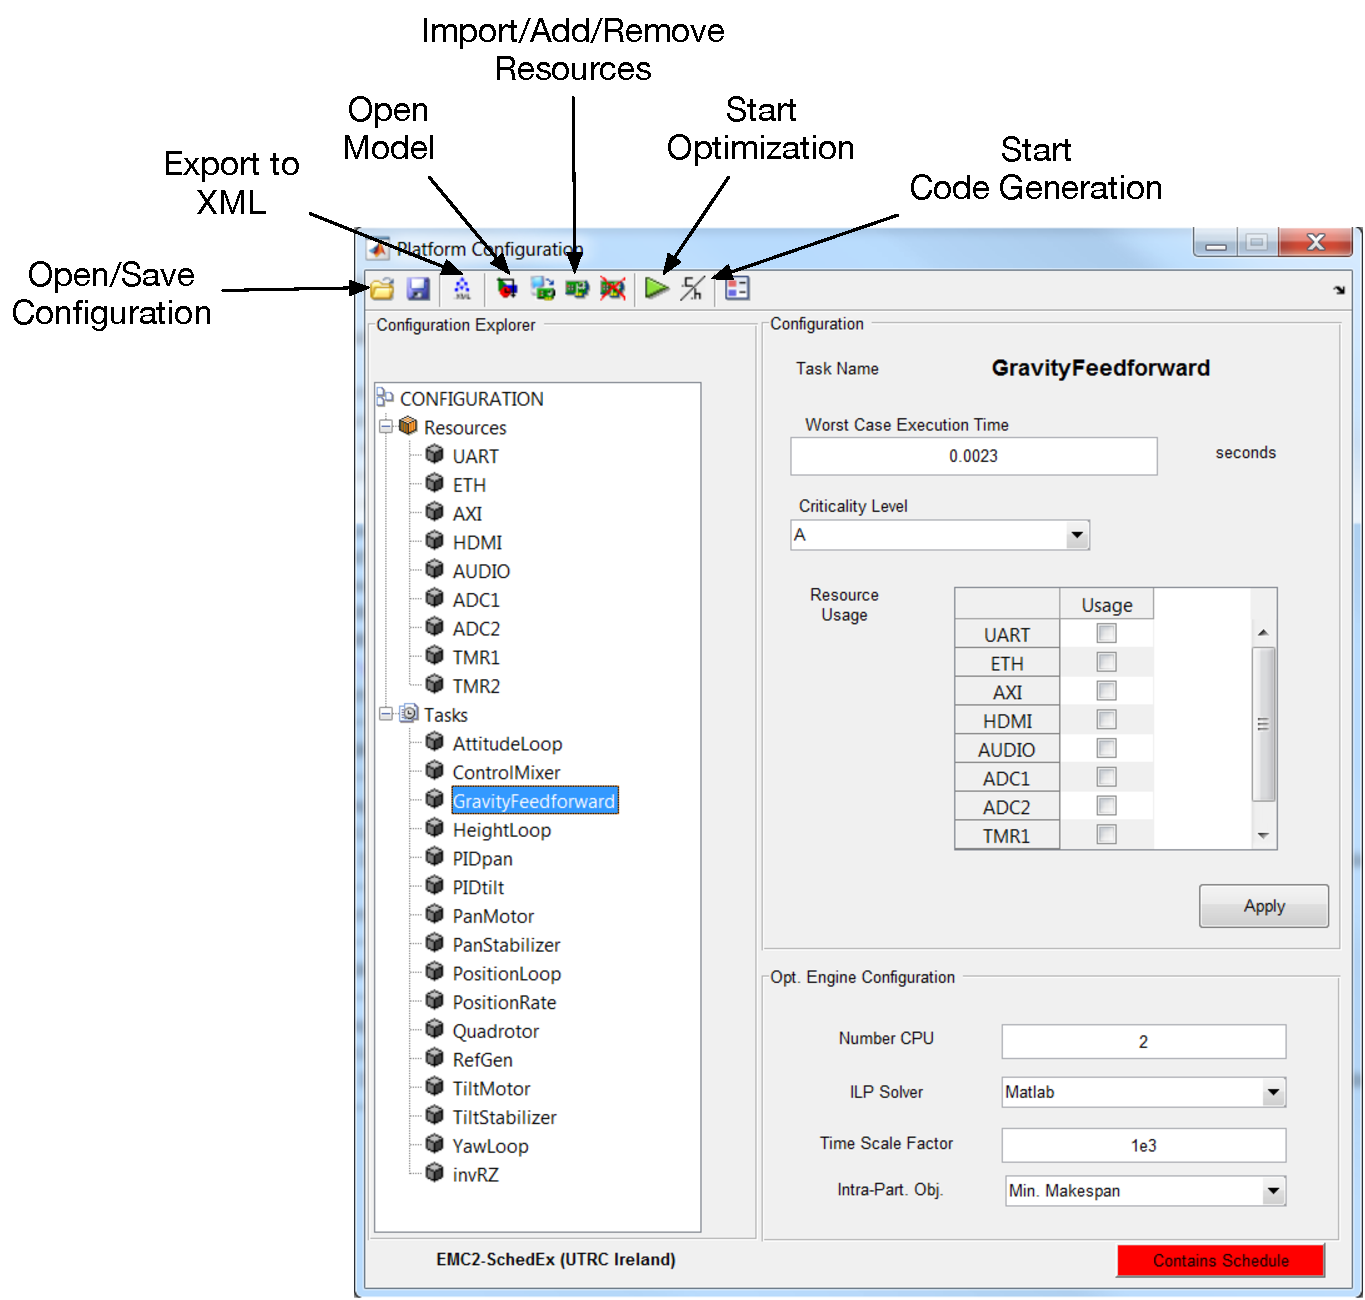
\includegraphics[width=0.6\textwidth]{PlatformConfiguration}
\caption{Tool Graphic User Interface (GUI)}
\label{fig:GUI}
\end{figure}
Here the designer can configure all the additional parameters that are required for each task. In particular, he can add all the resources on the platform, set up the optimization engine and specify for each task:
\begin{enumerate}
\item The Worst-Case Execution Time
\item The Criticality level (A to E)
\item The Resources the task uses
\end{enumerate}
In our example, the tasks are configured as shown in table \ref{tab:taskset}. The WCETs are randomly selected to make the task-set schedulable, otherwise, the inter-partition optimization problem states that no feasible solution is available.
\begin{table}
\begin{center}
\begin{tabular}{llcccc}  
\toprule
Task ID & Task Name    & Period & WCET & Criticality & Resources \\
\midrule
1  & AttitudeLoop      	& $0.1$  &	$9.135\cdot10^{-4}$     & A	& --\\
2  & ControlMixer     	& $0.1$  & 	$9.8412\cdot10^{-4}$    & A	& --\\
3  & GravityFeedforward & $0.1$  & 	$8.7592\cdot10^{-4}$    & A	& AXI \\
4  & HeightLoop      	& $0.1$  & 	$0.0012$			    & A	& AXI \\
5  & PIDpan      		& $0.05$ & 	$9.7148\cdot10^{-4}$    & B	& --\\
6  & PIDtilt      		& $0.05$ & 	$8.5084\cdot10^{-4}$    & B	& --\\
7  & PanMotor      		& $0.05$ & 	$5.4351\cdot10^{-4}$    & B	& AXI, ADC1\\
8  & PanStabilizer     	& $0.05$ &	$5.6589\cdot10^{-4}$    & B	& --\\
9  & PositionLoop      	& $0.1$  & 	$9.9352\cdot10^{-4}$    & A	& UART \\
10 & PositionRate      	& $0.1$  & 	$5.9584\cdot10^{-4}$    & A	& --\\
11 & Quadrotor      	& $0.01$ & 	$0.0033$			    & A	& AXI \\
12 & RefGen      		& $0.05$ & 	$4.8490\cdot10^{-4}$    & B	& UART \\
13 & TiltMotor      	& $0.05$ &	$4.0925\cdot10^{-4}$    & B	& AXI, ADC2\\
14 & TiltStabilizer     & $0.05$ & 	$9.0944\cdot10^{-4}$    & B	& --\\
15 & YawLoop      		& $0.1$  &	$8.2928\cdot10^{-4}$    & A	& --\\
16 & invRZ      		& $0.1$  &	$9.5648\cdot10^{-4}$    & A	& --\\
\bottomrule
\end{tabular}
\caption {Example Model Task-set}
\label{tab:taskset}
\end{center}
\end{table}
The task-set will be allocated on a dual-core processor and scheduled minimizing the makespan.

\subsection{Feedthrough relationships}
To fully understand the resulting functional model it is important to highlight the feedthrough relationship among ports of each subsystem. In figure \ref{fig:feedthrough} are shown all the paths. 
\begin{figure}[htbp] 
\centering    
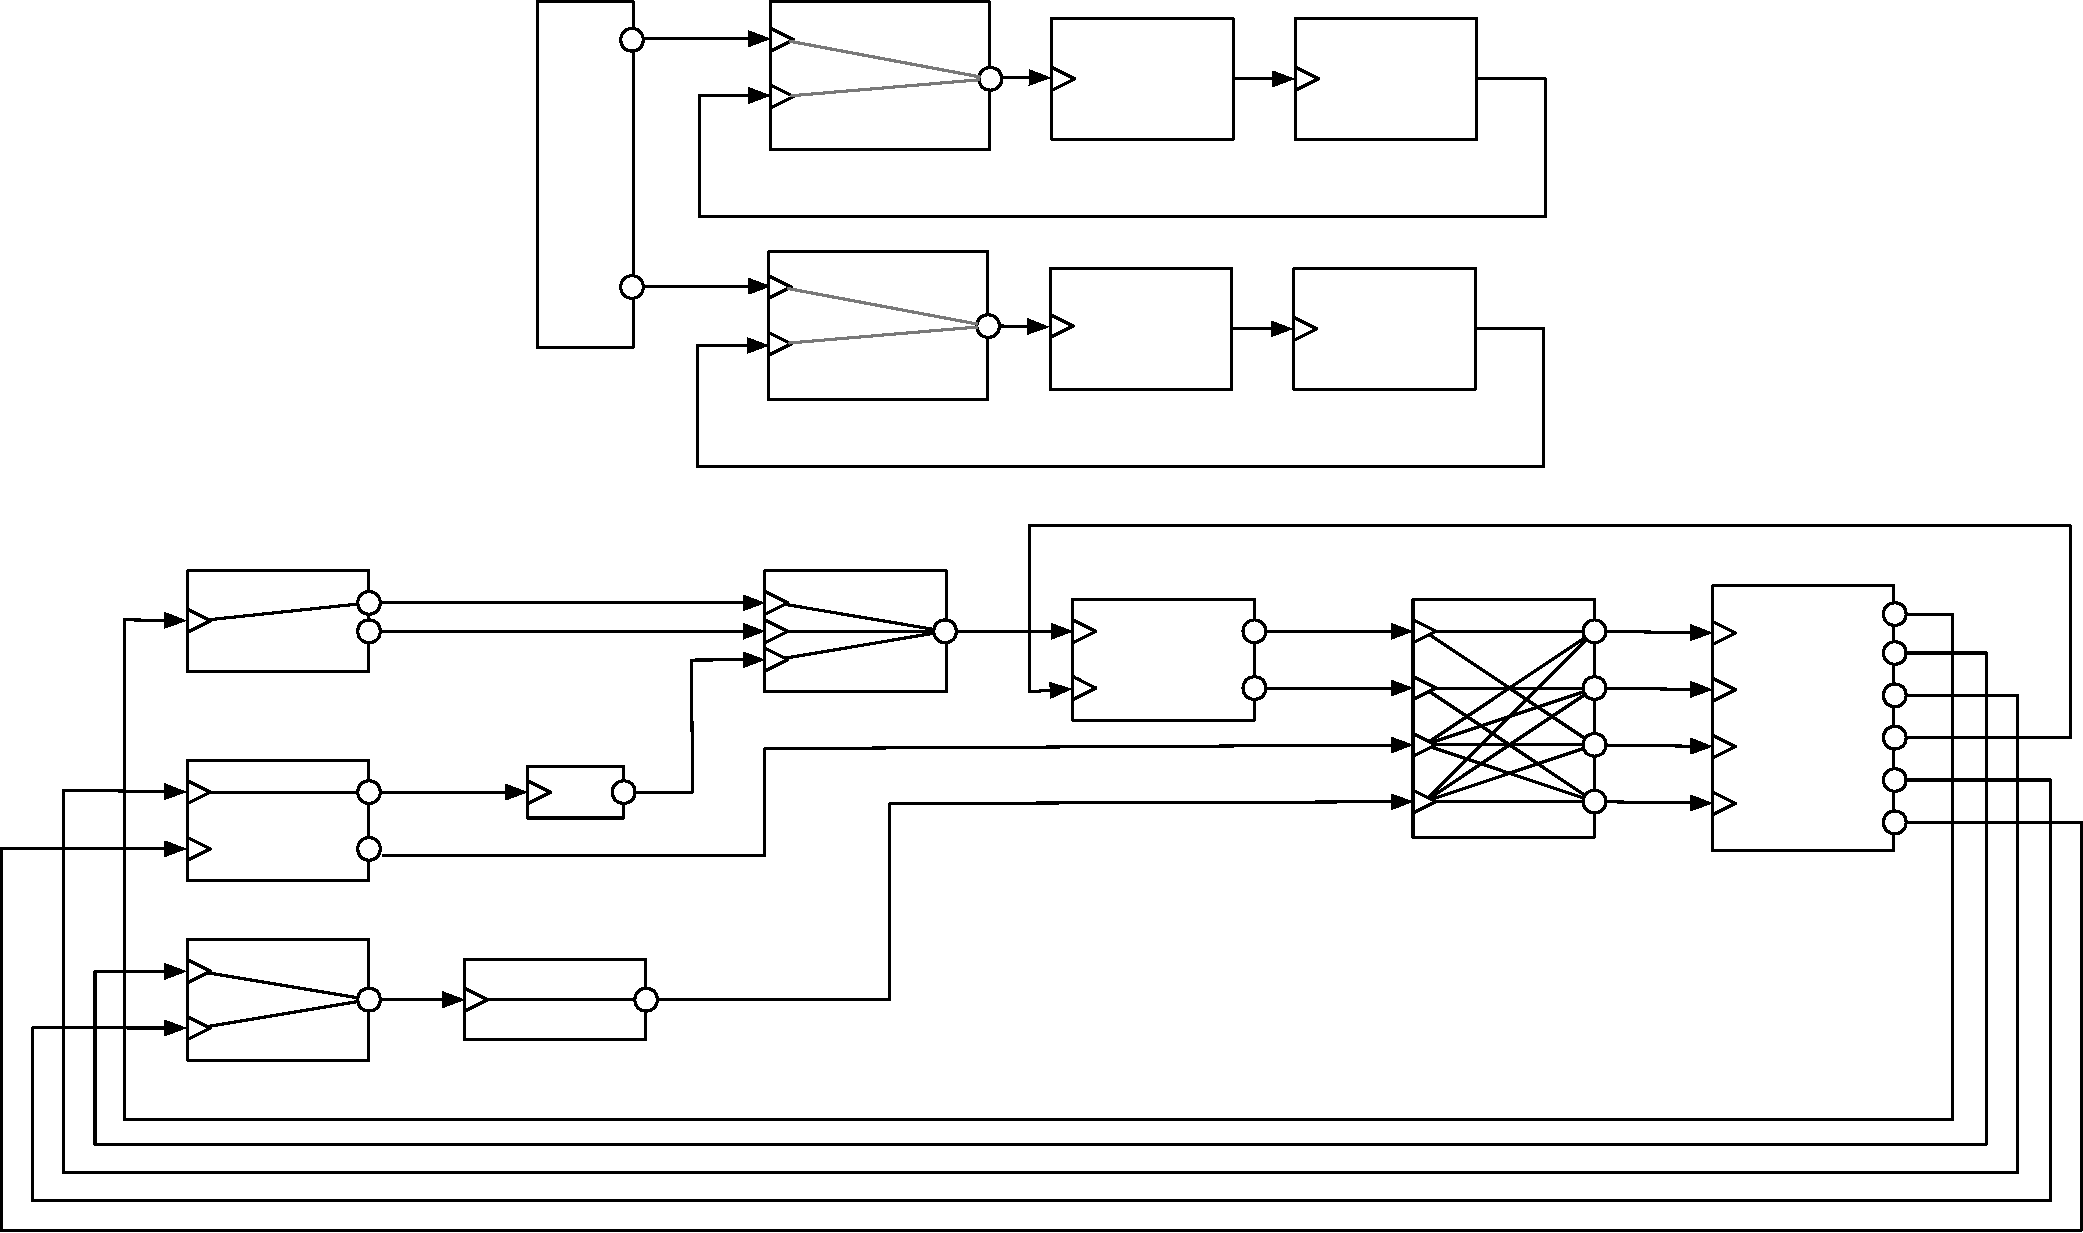
\includegraphics[width=0.7\textwidth]{FeedRelationships}
\caption{Feedthrough Relationships}
\label{fig:feedthrough}
\end{figure}
This relationship is automatically extracted from the model by a Matlab script and used to build the functional model.

%********************************** % Section  **************************************
\section{Functional Model Extraction}
Once the configuration is complete (i.e. WCET, Resources and Criticality), the system designer can start the scheduling process. The first step is the DAG extraction, which is transparent to the designer. Indeed, it is extracted  as soon as the GUI (or the model) is opened. The Direct-Acyclic Graph representing the task-set is shown in figure \ref{fig:extaskset}.
\begin{figure}[htbp] 
\centering    
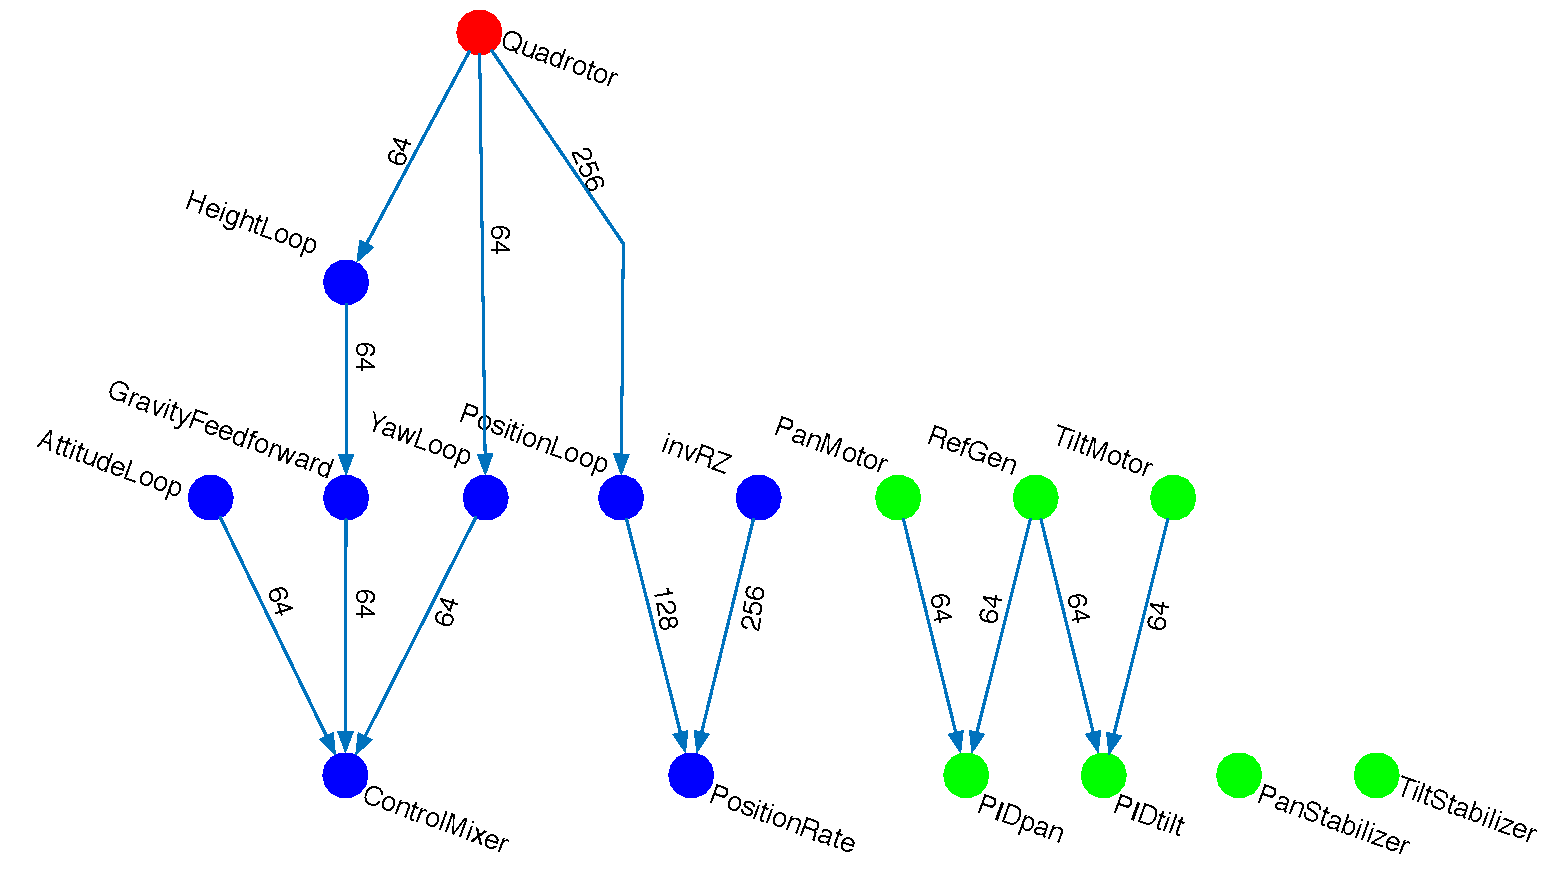
\includegraphics[width=0.9\textwidth]{Taskset}
\caption{Example Functional model - Task-set}
\label{fig:extaskset}
\end{figure}
Each color represent a different sample time, the edges the dependency among tasks. From the Simulink model, all the lines connecting two blocks where the input port of the destination block is not in a feedtrough relationship, has disappeared. This is the representation of the model used by the partitioning and scheduling algorithm.

%********************************** % Section  **************************************
\section{Scheduling}
The DAG, enriched with the information manually configured by the designer is the main input for the partitioning and scheduling algorithm. As already explained in section \ref{sec:DevelopedFramework}, the scheduling process is made by three phases: \begin{enumerate}
\item Partitioning
\item Intra-Partition Scheduling
\item Inter-Partition Scheduling
\end{enumerate}


\subsection{Partitioning}
The partitioning algorithm implements some form of robust partitioning of the task-set graph, the result of this step is figure \ref{fig:pdag} and is called P-DAG. While grouping tasks in partitions, some edge in the task-set cut the boundary of the partition, this edge represents a dependency among two partitions.
\begin{figure}[htbp] 
\centering    
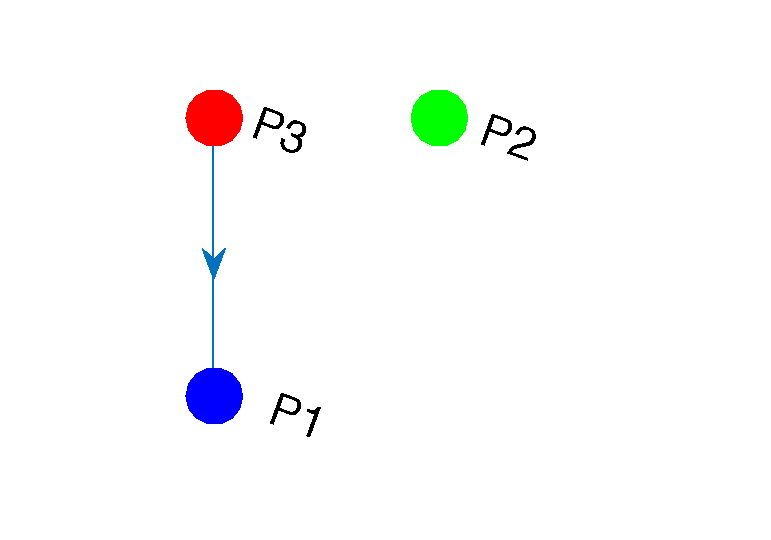
\includegraphics[width=0.3\textwidth]{PDAG}
\caption{Partition Graph, P-DAG}
\label{fig:pdag}
\end{figure}
All the edges in the P-DAG represent the partial order of execution imposed by the flow preservation requirement. The how tasks are redistributed in partitions is shown in table \ref{tab:partitions}.
\begin{table}
\begin{center}
\begin{tabular}{llc}  
\toprule
Partition & Tasks & Period \\
\midrule
P1  & 1,2,10,16,3,4,9,15 & $0.1$\\
P2  & 5,6,7,8,12,13,14 & $0.05$\\
P3  & 11 & 0.01\\
\bottomrule
\end{tabular}
\caption {Partitions}
\label{tab:partitions}
\end{center}
\end{table}

% \begin{figure}
%   \begin{subfigure}{1\textwidth}
%     \centering
%     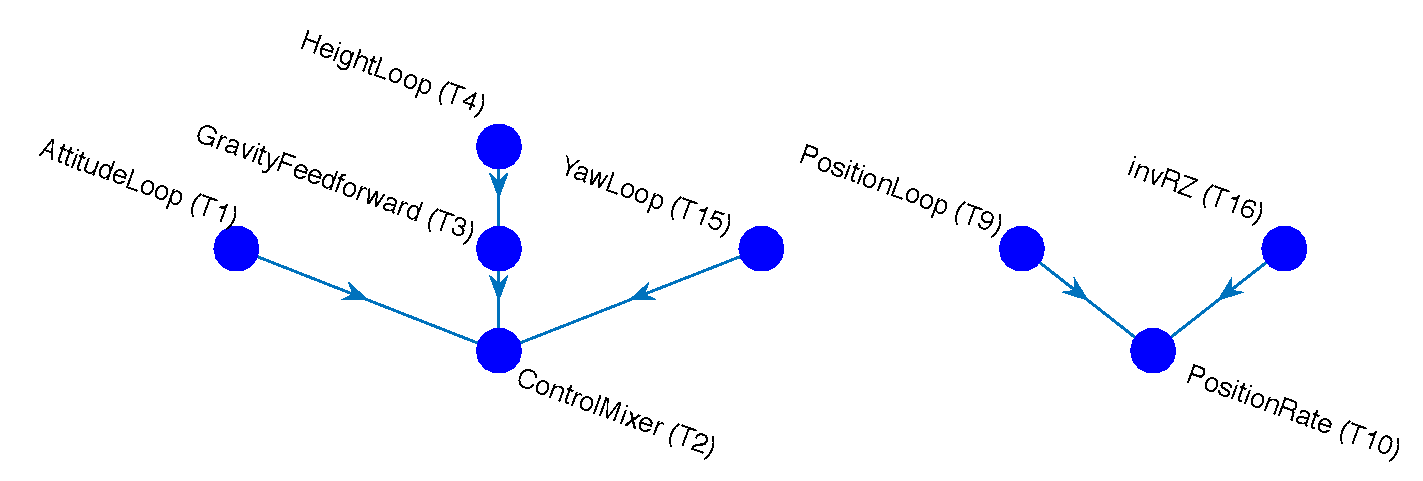
\includegraphics[width=1.0\textwidth]{TDAG1}
%     \caption{T-DAG Partition 1}
%     \label{fig:tdag1}
%   \end{subfigure}
%   \begin{subfigure}{1\textwidth}
%     \centering
%     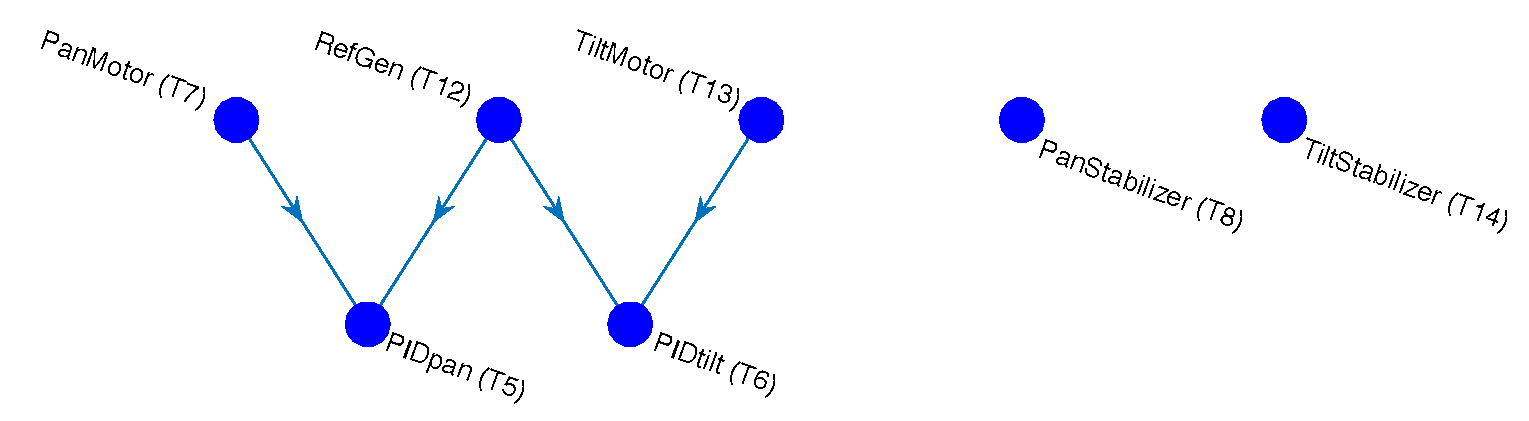
\includegraphics[width=1.0\textwidth]{TDAG2}
%     \caption{T-DAG Partition 2}
%     \label{fig:tdag2}
%   \end{subfigure}
%   \begin{subfigure}{1\textwidth}
%   \centering
%     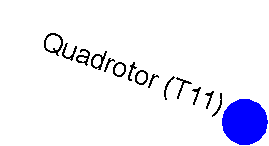
\includegraphics[width=0.2\textwidth]{TDAG3}
%     \caption{T-DAG Partition 3}
%     \label{fig:tdag3}
%   \end{subfigure}
%   \caption{T-DAGs}
%   \label{fig:tdag}
% \end{figure}

\subsection{Intra-Partition Scheduling}
Each node of the P-DAG represent a partition so, each partition contains some tasks, the subgraph of the task-set graph related to a partition is called T-DAG. % (figure \ref{fig:tdag}).
The allocation and scheduling of each T-DAG is called \emph{Intra-Partition Scheduling}. For each T-DAG the MILP optimization problem is solved on the relative subgraph (table \ref{tab:milp}). Note that task three and four cannot execute in parallel in partition one because both use the AXI interface (resource). Similarly, task 7 and 13 cannot execute in parallel in partition 2. This constraint is encoded in the incompatibility matrix.
\begin{table}
\begin{center}
\begin{tabular}{cccc}  
\toprule
Partition & Solution Time & Number of Constraints & Number of Variables (continuous) \\
\midrule
P1  & 0.34 seconds & 313 & 161(16)\\
P2  & 0.09 seconds & 237 & 127(14)\\
P3  & 0.03 seconds & 3 	 & 6(2)\\
\bottomrule
\end{tabular}
\caption {MILP formulations}
\label{tab:milp}
\end{center}
\end{table}
The resulting schedule is depicted in figure \ref{fig:intra}.

\begin{figure}
  \begin{subfigure}{0.8\textwidth}
    \centering
    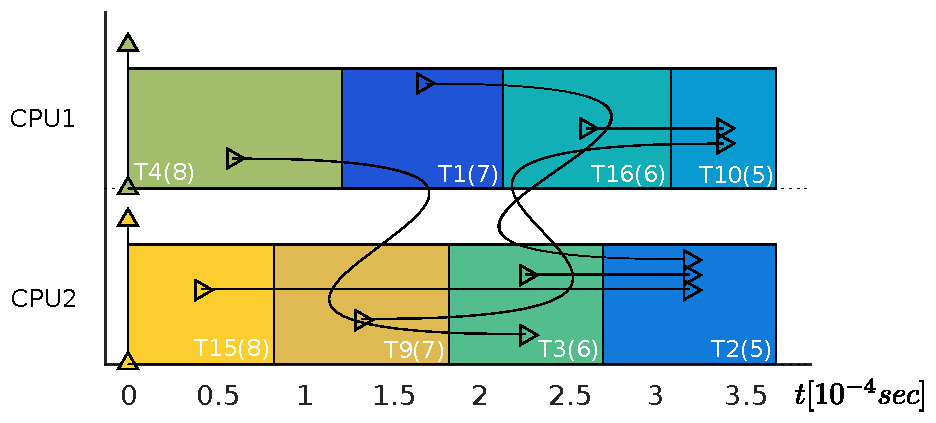
\includegraphics[width=1.0\textwidth]{intraP1}
    \caption{Partition 1 Schedule}
    \label{fig:intraP1}
  \end{subfigure}
  \begin{subfigure}{0.8\textwidth}
    \centering
    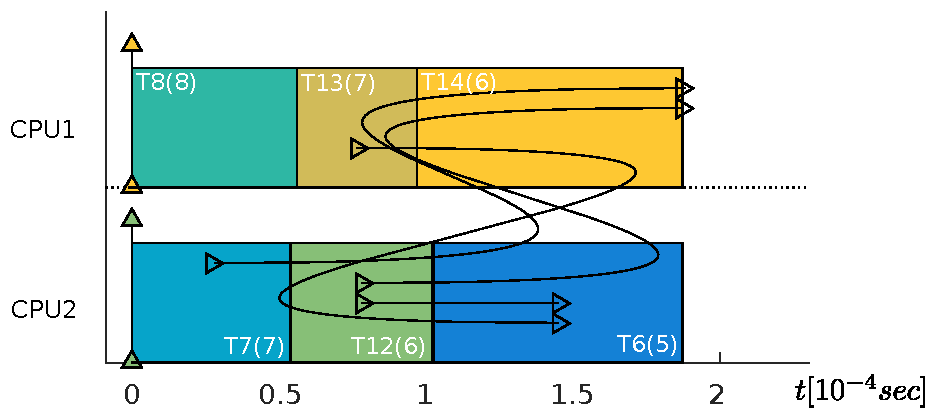
\includegraphics[width=1.0\textwidth]{intraP2}
    \caption{Partition 2 Schedule}
    \label{fig:intraP2}
  \end{subfigure}
  \begin{subfigure}{0.8\textwidth}
  \centering
    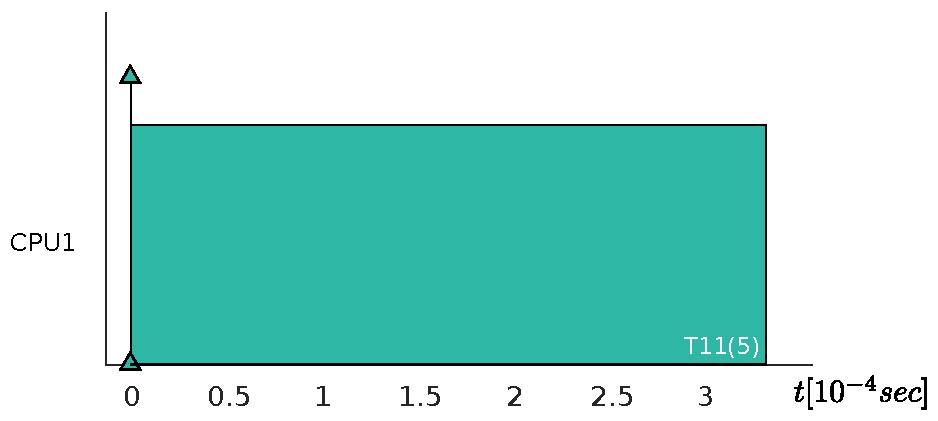
\includegraphics[width=1.0\textwidth]{intraP3}
    \caption{Partition 3 Schedule}
    \label{fig:intraP3}
  \end{subfigure}
  \caption{Intra-Partition Schedule}
  \label{fig:intra}
\end{figure}

Again, the arrows among tasks represent the dependency relationship.

%PARTITION 1
% V 	= [1,		2,			10,		16,			3,			4,	  9,			15]
% CPU 	= 1     	2     		1     	1     		2     		1     2     		2
% Start = 0.0012    0.0027    0.0031    0.0021    0.0018         0    0.0008         0
%PARTITION 2
% V 	= [5,		6,				7,		8,		12,		13,			14]
% CPU 	=  1     	2     			2		 1     2     	1     		1
% Start = 0.0019    0.0010         0         0    0.0005    0.0006    0.0010
%PARTITION 3
% V 	= 11
% CPU 	=  1
% Start = 0

\subsection{Priority Assignment}
When a schedule is obtained another optimization problem assigns priorities to each task as described in section \ref{sec:priorityassignment}. In particular figure \ref{fig:PriorityAssignment} shows that some priority value can be left unused for allowing some low priority task to be executed, in this example we use an offset of 5 for solving the optimization problem. The resulting assignment is shown in figure \ref{fig:intra}, tasks priorities are enclosed by parenthesis.
%	  [1,    2,    10,  16,	   3,    4,    9,    15]
%P1 => 7     5     5     6     6     8     7     8
%     [5,    6,    7,    8,    12,   13,   14]
%P2 => 5     5     7     8     6     7     6
%P3 => 5

\subsection{Inter-Partition Scheduling}
The final step of the scheduling process is the inter-partition scheduling. As described in section \ref{interpartition}, the Bratley algorithm is exploited to find the optimal solution. To include precedence constraints and periodicity, the P-DAG must be factorized. In the current example the Hyper-period is $0.1$ seconds, so, inside this interval partition $P_1$ execute only one, partition $P_2$ execute twice and partition $P_3$ execute 10 times. The resulting factorized P-DAG is shown in figure \ref{fig:fPDAG}.
\begin{figure}[htbp] 
\centering    
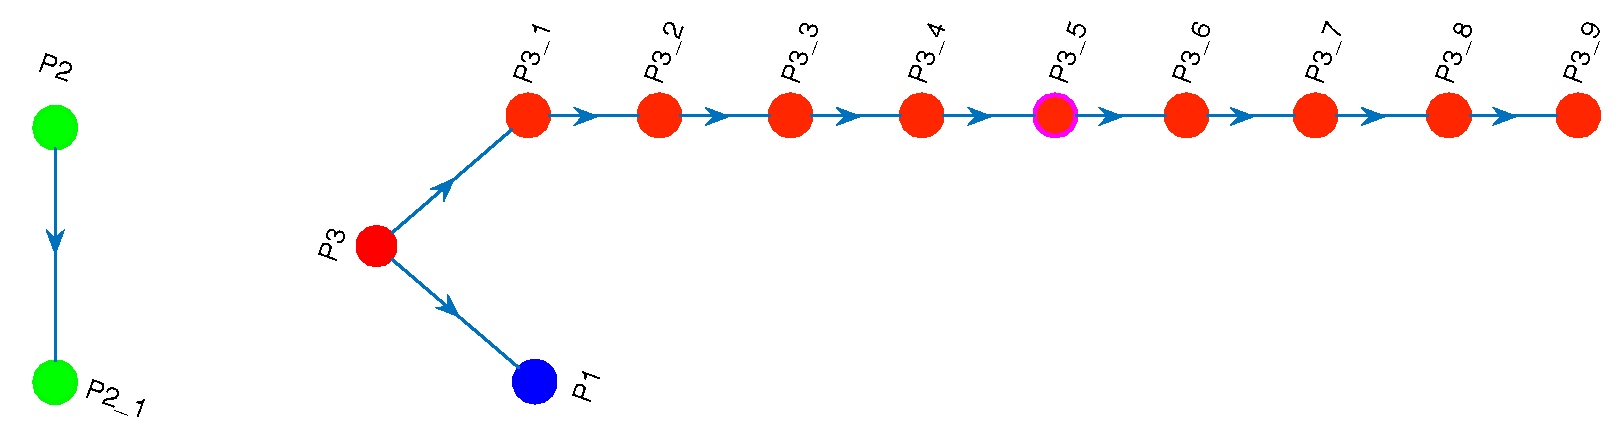
\includegraphics[width=0.8\textwidth]{fPDAG}
\caption{Factorized Partition Graph}
\label{fig:fPDAG}
\end{figure}

Thanks to Lemma \label{eq:precedenceLemma}, has been proven that if release times and deadlines are consistent with the precedence relation, then any normal one-processor schedule that satisfies the release times and deadlines must also obey the precedence relation, so a release time and a due date can be assigned to each partition according to formula \ref{eq:precedence}. They are summarized in table \label{tab:partitionset}.

\begin{table}
\begin{center}
\begin{tabular}{lcccc}  
\toprule
Partition ID & WCET &  Release Time & Due Date & Activation \\
\midrule
$P_1$ & 0.0037 & 0.0033 & 0.1 &0.0052\\
$P_2$ & 0.0019 & 0 & 0.05 & 0\\
$P_3$ & 0.033 & 0 & 0.01 & 0.0019\\
$P_2^1$ & 0.0019 & 0.05 & 0.01 & 0.05\\
$P_3^1$ & 0.033 & 0.01 & 0.02 & 0.01\\
$P_3^2$ & 0.033 & 0.02 & 0.03 & 0.02\\
$P_3^3$ & 0.033 & 0.03 & 0.04 & 0.03\\
$P_3^4$ & 0.033 & 0.04 & 0.05 & 0.04\\
$P_3^5$ & 0.033 & 0.05 & 0.06 & 0.0519\\
$P_3^6$ & 0.033 & 0.06 & 0.07 & 0.06\\ 
$P_3^7$ & 0.033 & 0.07 & 0.08 & 0.07\\
$P_3^8$ & 0.033 & 0.08 & 0.09 & 0.08\\ 
$P_3^9$ & 0.033 & 0.09 & 0.11 & 0.09\\
\bottomrule
\end{tabular}
\caption {Partition-set}
\label{tab:partitionset}
\end{center}
\end{table}

The Partition-set in table \ref{tab:partitionset} (except the last column) feeds the Bratley algorithm that enumerate all the possible feasible solution and select the optimal one. Int inter-partition schedule is shown in figure \ref{fig:inter}. All the activation times for each partition is listed in table \ref{tab:partitionset} (last column).
\begin{figure}[htbp] 
\centering    
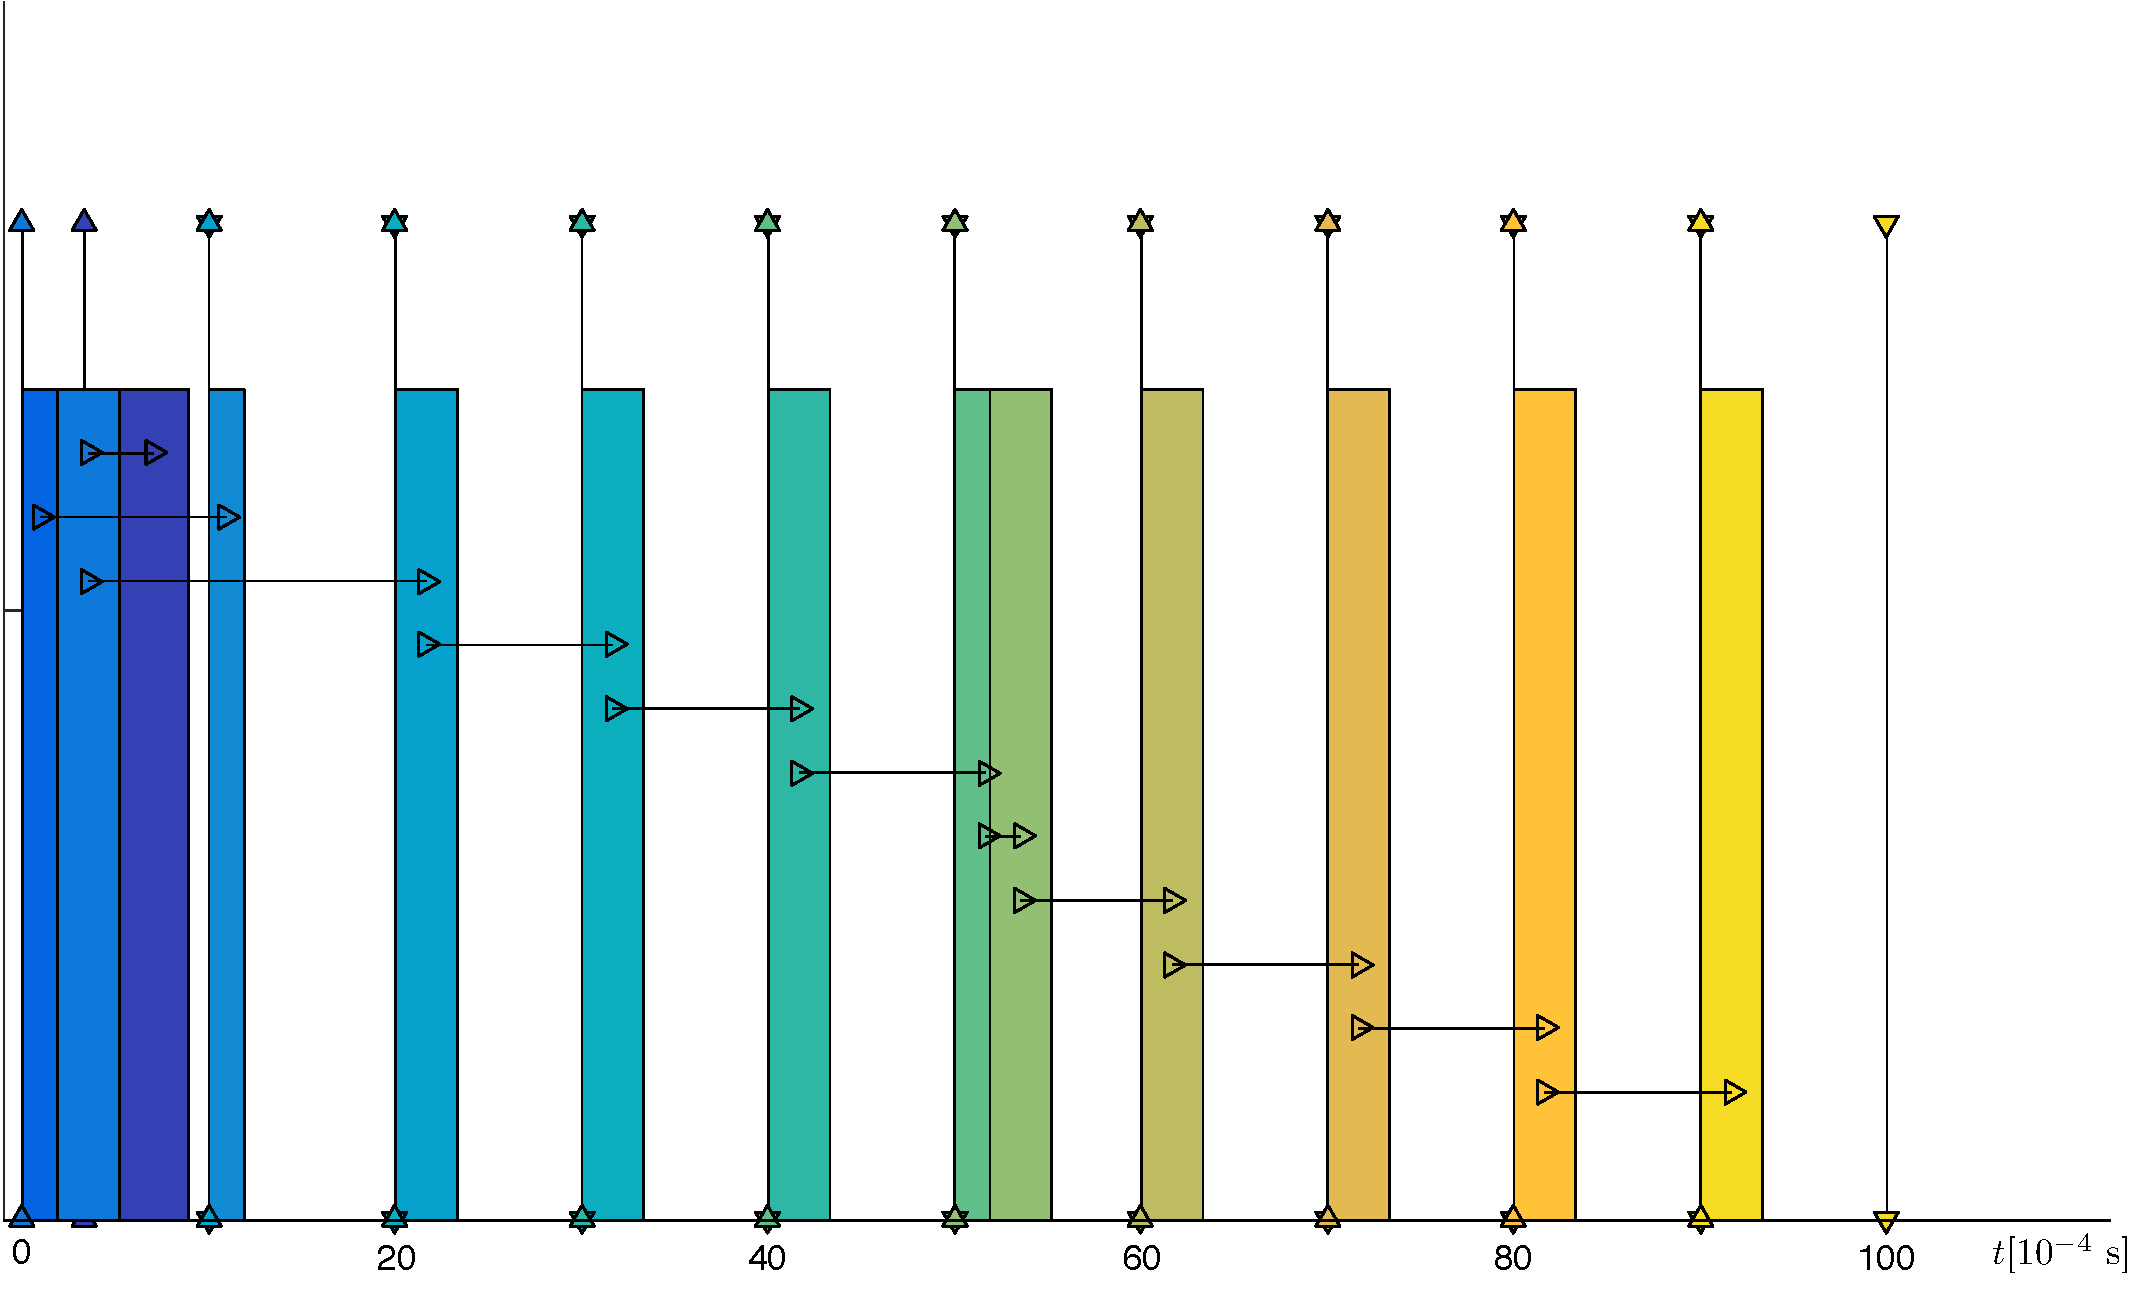
\includegraphics[width=0.8\textwidth]{inter}
\caption{Inter-Partition Schedule}
\label{fig:inter}
\end{figure}

\subsection{Theoretical Performance}
In order to assert how well the model can be run on multi-core, various metrics need to be defined first. Using the right metric makes it possible to determine how one would benefit from parallelizing the model as well as how various actions like changing the model changed the performance. In this work only widely used performance metrics for parallel systems are used, since a system’s performance is the main motivation behind switching to a multi-core architecture. These include the makespan (mentioned in the previous section), the \emph{speed-up} and the \emph{efficiency} \cite{grama2003}.

\paragraph{} When used for parallel systems, the makespan can be divided into two metrics: \emph{sequential makespan} and \emph{parallelized makespan}. The sequential makespan is the execution time required by the task-set to execute on a single-core. Used together with the parallelized makespan, which is the execution time on multiple cores, various other metrics like the speed-up can be calculated. 
\par Speed-up is defined as the ratio of the elapsed time when executing a program on a single processor (the sequential makespan $W_1$) to the execution time when $p$ processors are available (the parallelized makespan $W_p$)\cite{speedup}. Throughout this work, it is defined as,
\begin{equation}
    S(p) = \frac{W_1}{W_p}
\end{equation}
With this metric it is possible to assert how the execution time of a system as improved by changing the number of cores. In theory, the speed-up can never exceed the number of processors $p$, the best case. This introduces the \emph{efficiency}. It is defined as the average utilization of the $p$ allocated processors \cite{speedup}. This value tells us how much average speedup is gained by investing in $p$-core, enabling us to declare how worthwhile a multi-core system is for a given system. Formally it is defined as:
\begin{equation}
    E(p)=\frac{S(p)}{p}
\end{equation}
Efficiency can only reach values between 0 and 1. Programs with linear speed-up have an efficiency of 1. It is worth mentioning that in practice, linear speed-up is not achievable in practice since adding more processors increases the communication time between processors as well as the time waiting for shared resources to unlock, which are not considered in this model.

\paragraph{} For each partition both the speed-up and the efficiency can be computed, they are summarized in table \ref{tab:performance}.
\begin{table}
\begin{center}
\begin{tabular}{lcccc}  
\toprule
Partition & Speed-up & Efficiency \\
\midrule
$P_1$ & 1.9927 & 0.99\\
$P_2$ & 1.9927 & 0.99\\
$P_3$ & 1 & 0.5\\
\bottomrule
\end{tabular}
\caption {Performance}
\label{tab:performance}
\end{center}
\end{table}
The MILP problem, since finds the optimal solution, does a good job in exploiting all the possible time in the partition on both available cores. There is no idle time in the intra-partition schedule (see fig. \ref{fig:intra}) so the speed-up is approximately 2 for partition one and partition two.

\paragraph{} At this point all the information about the scheduling are known, so the code generation process can be started.

%********************************** % Section  **************************************
\section{Code Generation}
Once a feasible schedule is available, the system designer can start the code generation process pressing the button \emph{Start Code Generation} in the framework GUI. This operation will save the current schedule to an XML file and call the code generation entry point. After parsing the file, the model is adapted to the communication model described in the exported configuration.

\subsection{Adapted model}
As described in section \ref{sec:modelAdapt}, before generating the C code, all the subsystem ports that are communication data to subsystem assigned to another partition needs to be substituted with the correct operation on a Sampling Port. This is automatically done by the script after parsing the configuration file. In figure \ref{fig:adaptedModel} it is possible to see that all the lines connecting \verb|Quadrotor| with all other blocks disappeared. As expected, all partitions are isolated one from each other, meaning that there are no lines between blocks.
\begin{figure}[htbp] 
\centering    
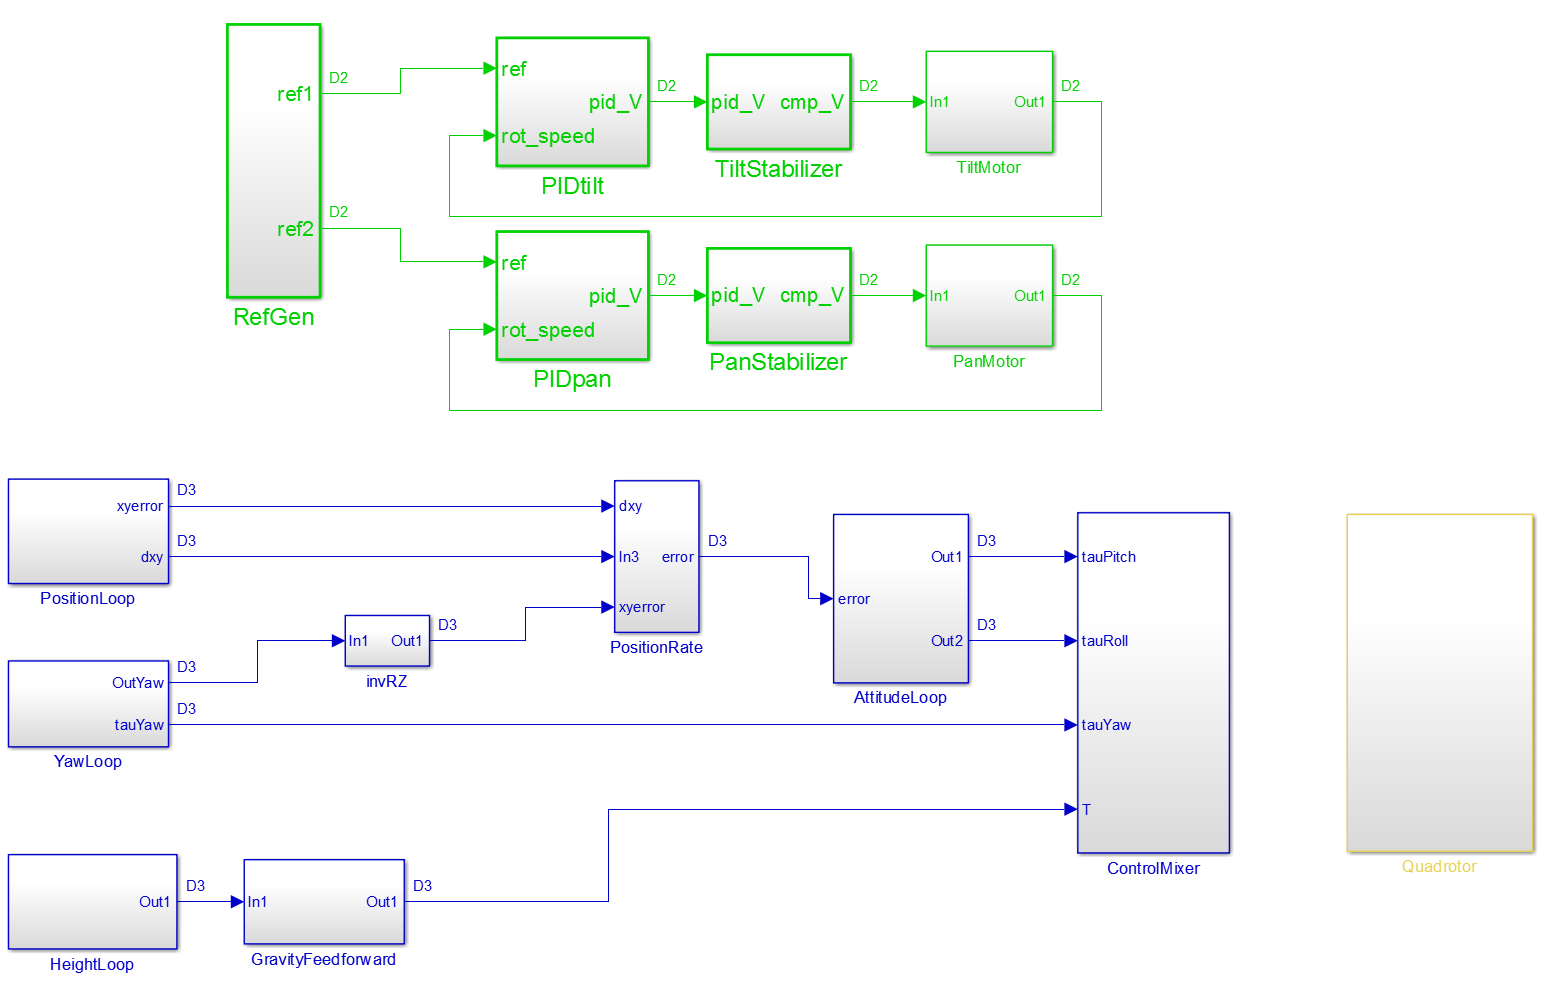
\includegraphics[width=1\textwidth]{AdaptedModel}
\caption{Adapted Model}
\label{fig:adaptedModel}
\end{figure}
The next step generates the C code for each block.

\subsection{Partition Main Threads}
To generate the code of each block is used the System Target file described in section \ref{slexSTF}. It generates the C code for each single block as Embedded Coder would do, also it generates an XML file describing the structure of the code. When all the blocks have been generated, all these XML files are collected and parsed to correctly generate the code of each partition.

\paragraph{} As described in section \ref{nativeprocess}, each Native PikeOS process is made by the main thread and all the thread composing that partition. The code for this two entities is inside separate files for each partition, e.g. \verb|P1_main.c|, \verb|P2_main.c|, \verb|P3_main.c|. As an example let consider the code of the main thread of partition one.
\lstinputlisting[language=C]{Chapters/SrcCode/P1_main.c}
The threads it creates matches the ones in \ref{tab:partitions} for $P_1$ with the priorities in figure \ref{TBD}. It also initializes some spinlocks, one for each inter-core communications, each of them can be graphically seen in figure \ref{fig:intra} by edges between tasks scheduled on different cores.
\par After creating and letting each thread to execute its initialization code (lines 15-30) the main thread enters an infinite loop where each thread is resumed every time a new period starts.

\paragraph{} As an example let consider the code of the thread about \verb|AttitudeLoop| (thread 1), this is interesting because is used both data directly from a thread in the same process and data coming from the sampling port. The code of this thread is the following.
\begin{lstlisting}[language=C]
static void AttitudeLoop_thread(void){
      P4_e_t rc;

      AttitudeLoop_initialize();
      vm_cprintf("AttitudeLoop initialized...\n");
      p4_thread_stop(P4_THREAD_MYSELF);

      /* Continous loop */
	for(;;){
		/* Input update */
		AttitudeLoop_U.pitchrolldmd[0] = PositionRate_Y.error[0];
		AttitudeLoop_U.pitchrolldmd[1] = PositionRate_Y.error[1];

		/* Step */
		AttitudeLoop_step();

		/* Unlock Spinlocks */
		P4_spin_unlock(&AttitudeLoop1_ControlMixer1_spinlock);
		p4_spin_unlock(&AttitudeLoop2_ControlMixer2_spinlock);

		/* Wait for next period */
		p4_thread_stop(P4_THREAD_MYSELF);
	}

	/* Terminate - Never Reached */
	AttitudeLoop_terminate();
}
\end{lstlisting}
On lines 11-12 it takes the data directly from the shared structure. The data from the sampling port are retrieved inside the \verb|AttitudeLoop_step()| because the code for reading from the port is generated directly from RTW thanks to the Custom Block. Indeed, inside the file \verb|AttitudeLoop.c|, the following code appears.
\begin{lstlisting}[language=C]
P4_e_t rc1 = vm_sport_read(&AttitudeLoop_sport1_d, &AttitudeLoop_B.PitchRoll[0],
    4*sizeof(real_T), &read_size, &validity);
\end{lstlisting}
When the step function of the subsystem has been executed, the successor that is executing on another core can be notified. For this reason, two spinlocks are unlocked on lines 18-19 notifying the thread \verb|ControlMixer| that the data are available. Finally, the thread goes in the STOPPED state on line 22, waiting for the next activation from the main thread.

\subsection{Integration Project Snippets}
Out of the code generation process, some XML snippets are generated to help the configuration of the Integration Project. For the sake of conciseness, they are nor reported here because they are quite long. For example, schedule scheme is 64 lines long since in every moment there is at least one partition active, this means that for each gap in the schedule of figure \ref{fig:inter} the \TP{0} is statically allocated for non-real time operation (e.g. muxa and other services).

